\documentclass[border=4pt]{standalone}
\usepackage{tikz}
\usetikzlibrary{calc,shapes.multipart}
\begin{document}
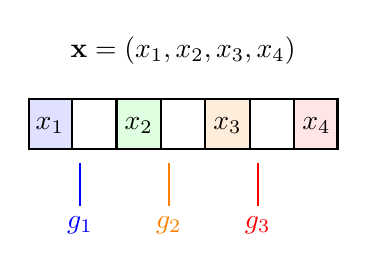
\begin{tikzpicture}
  \node[
    rectangle split,
    rectangle split horizontal,
    rectangle split parts=7,
    rectangle split empty part width=1pt,
    rectangle split empty part width=2pt,
    rectangle split empty part width=3pt,
    rectangle split empty part height=.5ex,
    rectangle split empty part height=2ex,
    rectangle split empty part depth=.5ex,
    rectangle split empty part depth=1ex,
    rectangle split part fill={blue!12,white,green!12,white,orange!14,white,red!10},
    rectangle split part align=base,
    inner sep=2.5pt,
    draw,
    thick
  ] (vector) {$x_1$\nodepart{two}\nodepart{three}$x_2$\nodepart{four}\nodepart{five}$x_3$\nodepart{six}\nodepart{seven}$x_4$};
  \draw[blue,thick] ($(vector.two)+(0,-.42)$) -- ++(0,-.55) node[below] {$g_1$};
  \draw[orange,thick] ($(vector.four)+(0,-.42)$) -- ++(0,-.55) node[below] {$g_2$};
  \draw[red,thick] ($(vector.six)+(0,-.42)$) -- ++(0,-.55) node[below] {$g_3$};
  \node[above=3mm] at (vector.north) {$\mathbf{x}=(x_1,x_2,x_3,x_4)$};
\end{tikzpicture}
\end{document}
